% Options for packages loaded elsewhere
\PassOptionsToPackage{unicode}{hyperref}
\PassOptionsToPackage{hyphens}{url}
\PassOptionsToPackage{dvipsnames,svgnames,x11names}{xcolor}
%
\documentclass[
  10pt,
  ignorenonframetext,
  aspectratio=169]{beamer}
\usepackage{pgfpages}
\setbeamertemplate{caption}[numbered]
\setbeamertemplate{caption label separator}{: }
\setbeamercolor{caption name}{fg=normal text.fg}
\beamertemplatenavigationsymbolsempty
% Prevent slide breaks in the middle of a paragraph
\widowpenalties 1 10000
\raggedbottom
\setbeamertemplate{part page}{
  \centering
  \begin{beamercolorbox}[sep=16pt,center]{part title}
    \usebeamerfont{part title}\insertpart\par
  \end{beamercolorbox}
}
\setbeamertemplate{section page}{
  \centering
  \begin{beamercolorbox}[sep=12pt,center]{part title}
    \usebeamerfont{section title}\insertsection\par
  \end{beamercolorbox}
}
\setbeamertemplate{subsection page}{
  \centering
  \begin{beamercolorbox}[sep=8pt,center]{part title}
    \usebeamerfont{subsection title}\insertsubsection\par
  \end{beamercolorbox}
}
\AtBeginPart{
  \frame{\partpage}
}
\AtBeginSection{
  \ifbibliography
  \else
    \frame{\sectionpage}
  \fi
}
\AtBeginSubsection{
  \frame{\subsectionpage}
}
\usepackage{amsmath,amssymb}
\usepackage{lmodern}
\usepackage{iftex}
\ifPDFTeX
  \usepackage[T1]{fontenc}
  \usepackage[utf8]{inputenc}
  \usepackage{textcomp} % provide euro and other symbols
\else % if luatex or xetex
  \usepackage{unicode-math}
  \defaultfontfeatures{Scale=MatchLowercase}
  \defaultfontfeatures[\rmfamily]{Ligatures=TeX,Scale=1}
\fi
\usetheme[]{Singapore}
% Use upquote if available, for straight quotes in verbatim environments
\IfFileExists{upquote.sty}{\usepackage{upquote}}{}
\IfFileExists{microtype.sty}{% use microtype if available
  \usepackage[]{microtype}
  \UseMicrotypeSet[protrusion]{basicmath} % disable protrusion for tt fonts
}{}
\makeatletter
\@ifundefined{KOMAClassName}{% if non-KOMA class
  \IfFileExists{parskip.sty}{%
    \usepackage{parskip}
  }{% else
    \setlength{\parindent}{0pt}
    \setlength{\parskip}{6pt plus 2pt minus 1pt}}
}{% if KOMA class
  \KOMAoptions{parskip=half}}
\makeatother
\usepackage{xcolor}
\newif\ifbibliography
\usepackage{color}
\usepackage{fancyvrb}
\newcommand{\VerbBar}{|}
\newcommand{\VERB}{\Verb[commandchars=\\\{\}]}
\DefineVerbatimEnvironment{Highlighting}{Verbatim}{commandchars=\\\{\}}
% Add ',fontsize=\small' for more characters per line
\usepackage{framed}
\definecolor{shadecolor}{RGB}{48,48,48}
\newenvironment{Shaded}{\begin{snugshade}}{\end{snugshade}}
\newcommand{\AlertTok}[1]{\textcolor[rgb]{1.00,0.81,0.69}{#1}}
\newcommand{\AnnotationTok}[1]{\textcolor[rgb]{0.50,0.62,0.50}{\textbf{#1}}}
\newcommand{\AttributeTok}[1]{\textcolor[rgb]{0.80,0.80,0.80}{#1}}
\newcommand{\BaseNTok}[1]{\textcolor[rgb]{0.86,0.64,0.64}{#1}}
\newcommand{\BuiltInTok}[1]{\textcolor[rgb]{0.80,0.80,0.80}{#1}}
\newcommand{\CharTok}[1]{\textcolor[rgb]{0.86,0.64,0.64}{#1}}
\newcommand{\CommentTok}[1]{\textcolor[rgb]{0.50,0.62,0.50}{#1}}
\newcommand{\CommentVarTok}[1]{\textcolor[rgb]{0.50,0.62,0.50}{\textbf{#1}}}
\newcommand{\ConstantTok}[1]{\textcolor[rgb]{0.86,0.64,0.64}{\textbf{#1}}}
\newcommand{\ControlFlowTok}[1]{\textcolor[rgb]{0.94,0.87,0.69}{#1}}
\newcommand{\DataTypeTok}[1]{\textcolor[rgb]{0.87,0.87,0.75}{#1}}
\newcommand{\DecValTok}[1]{\textcolor[rgb]{0.86,0.86,0.80}{#1}}
\newcommand{\DocumentationTok}[1]{\textcolor[rgb]{0.50,0.62,0.50}{#1}}
\newcommand{\ErrorTok}[1]{\textcolor[rgb]{0.76,0.75,0.62}{#1}}
\newcommand{\ExtensionTok}[1]{\textcolor[rgb]{0.80,0.80,0.80}{#1}}
\newcommand{\FloatTok}[1]{\textcolor[rgb]{0.75,0.75,0.82}{#1}}
\newcommand{\FunctionTok}[1]{\textcolor[rgb]{0.94,0.94,0.56}{#1}}
\newcommand{\ImportTok}[1]{\textcolor[rgb]{0.80,0.80,0.80}{#1}}
\newcommand{\InformationTok}[1]{\textcolor[rgb]{0.50,0.62,0.50}{\textbf{#1}}}
\newcommand{\KeywordTok}[1]{\textcolor[rgb]{0.94,0.87,0.69}{#1}}
\newcommand{\NormalTok}[1]{\textcolor[rgb]{0.80,0.80,0.80}{#1}}
\newcommand{\OperatorTok}[1]{\textcolor[rgb]{0.94,0.94,0.82}{#1}}
\newcommand{\OtherTok}[1]{\textcolor[rgb]{0.94,0.94,0.56}{#1}}
\newcommand{\PreprocessorTok}[1]{\textcolor[rgb]{1.00,0.81,0.69}{\textbf{#1}}}
\newcommand{\RegionMarkerTok}[1]{\textcolor[rgb]{0.80,0.80,0.80}{#1}}
\newcommand{\SpecialCharTok}[1]{\textcolor[rgb]{0.86,0.64,0.64}{#1}}
\newcommand{\SpecialStringTok}[1]{\textcolor[rgb]{0.80,0.58,0.58}{#1}}
\newcommand{\StringTok}[1]{\textcolor[rgb]{0.80,0.58,0.58}{#1}}
\newcommand{\VariableTok}[1]{\textcolor[rgb]{0.80,0.80,0.80}{#1}}
\newcommand{\VerbatimStringTok}[1]{\textcolor[rgb]{0.80,0.58,0.58}{#1}}
\newcommand{\WarningTok}[1]{\textcolor[rgb]{0.50,0.62,0.50}{\textbf{#1}}}
\usepackage{graphicx}
\makeatletter
\def\maxwidth{\ifdim\Gin@nat@width>\linewidth\linewidth\else\Gin@nat@width\fi}
\def\maxheight{\ifdim\Gin@nat@height>\textheight\textheight\else\Gin@nat@height\fi}
\makeatother
% Scale images if necessary, so that they will not overflow the page
% margins by default, and it is still possible to overwrite the defaults
% using explicit options in \includegraphics[width, height, ...]{}
\setkeys{Gin}{width=\maxwidth,height=\maxheight,keepaspectratio}
% Set default figure placement to htbp
\makeatletter
\def\fps@figure{htbp}
\makeatother
\setlength{\emergencystretch}{3em} % prevent overfull lines
\providecommand{\tightlist}{%
  \setlength{\itemsep}{0pt}\setlength{\parskip}{0pt}}
\setcounter{secnumdepth}{-\maxdimen} % remove section numbering
\newenvironment{cols}[1][]{}{}

\newenvironment{col}[1]{\begin{minipage}{#1}\ignorespaces}{%
\end{minipage}
\ifhmode\unskip\fi
\aftergroup\useignorespacesandallpars}

\def\useignorespacesandallpars#1\ignorespaces\fi{%
#1\fi\ignorespacesandallpars}

\makeatletter
\def\ignorespacesandallpars{%
  \@ifnextchar\par
    {\expandafter\ignorespacesandallpars\@gobble}%
    {}%
}
\makeatother
\ifLuaTeX
  \usepackage{selnolig}  % disable illegal ligatures
\fi
\usepackage[]{natbib}
\bibliographystyle{plainnat}
\IfFileExists{bookmark.sty}{\usepackage{bookmark}}{\usepackage{hyperref}}
\IfFileExists{xurl.sty}{\usepackage{xurl}}{} % add URL line breaks if available
\urlstyle{same} % disable monospaced font for URLs
\hypersetup{
  pdftitle={Word and Document Embeddings},
  pdfauthor={Max Callaghan},
  colorlinks=true,
  linkcolor={Maroon},
  filecolor={Maroon},
  citecolor={Blue},
  urlcolor={blue},
  pdfcreator={LaTeX via pandoc}}

\title{Word and Document Embeddings}
\author{Max Callaghan}
\date{2022-10-20}

\begin{document}
\frame{\titlepage}

\hypertarget{objectives}{%
\section{Objectives}\label{objectives}}

\begin{frame}{Objectives}
\protect\hypertarget{objectives-1}{}
By now we have figured out how to \textbf{represent} texts using the
``bag of words'' model.

Today we will look at \textbf{word embeddings}, which are a basic
building block for understanding much of much modern NLP.
\end{frame}

\hypertarget{word-embeddings}{%
\section{Word embeddings}\label{word-embeddings}}

\begin{frame}[fragile]{Why do we need word embeddings?}
\protect\hypertarget{why-do-we-need-word-embeddings}{}
With the bag of words model, there are as many columns as there are
unique words, and each column is completely independent.

Consider the following two texts

\begin{verbatim}
"The acclaimed author penned novels based on her life"

"Nobel prize-winning writer writes autobiographical fiction"
\end{verbatim}

Are they similar? Would an bag of words model consider these similar
texts?
\end{frame}

\begin{frame}{Word similarity}
\protect\hypertarget{word-similarity}{}
Words themselves can be similar. A richer model will represent this
similarity.

If this works, then the sentence

The \textbf{cat} sat on the mat.

will be much more similar to the sentence

The \textbf{dog} sat on the mat.

than it will be to the sentence

The \textbf{carbon} sat on the mat.
\end{frame}

\begin{frame}{How can we find similar words}
\protect\hypertarget{how-can-we-find-similar-words}{}
The intuition is that similar words appear in similar contexts
\end{frame}

\begin{frame}[fragile]{Word embeddings}
\protect\hypertarget{word-embeddings-1}{}
\href{https://arxiv.org/abs/1310.4546}{Mikolov et al, 2013} developed a
very efficient way to learn word embeddings for very large vocabularies.

\medskip

Essentially, neural networks are trained on huge corpora to predict
words from context (Continuous Bag of Words - CBOW) or context from
words (Skip-gram)

\begin{cols}

\begin{col}{0.6\textwidth}
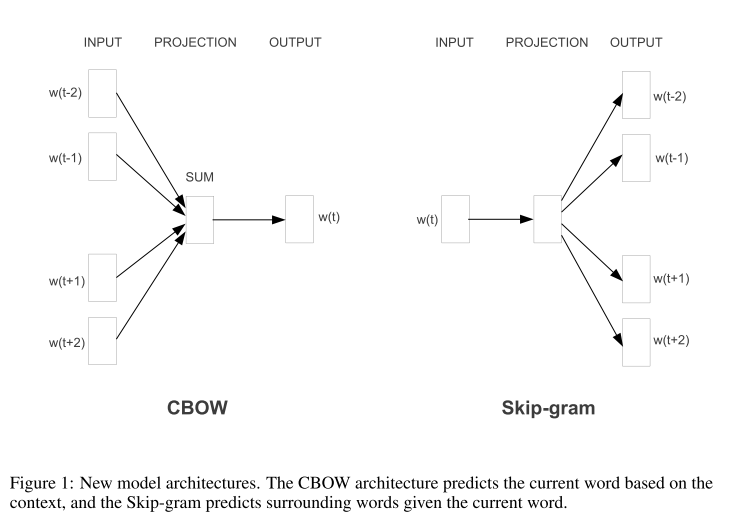
\includegraphics{images/cbow-skipgram.png}

\end{col}

\begin{col}{0.003\textwidth}
~

\end{col}

\begin{col}{0.4\textwidth}
from the sentence

\medskip

\begin{verbatim}
the cat sat on the mat
\end{verbatim}

\medskip

we would have the following context, target pairs to predict

\medskip

\texttt{({[}cat\ sat{]},\ the),\ ({[}the,\ sat,\ on{]},\ cat),\ ({[}the,\ cat,\ on,\ the{]},\ sat),\ ({[}cat,\ sat,\ the,\ mat{]},\ on),\ ({[}sat,\ on,\ mat{]},\ the),\ ({[}on,\ the{]},\ mat)}

\end{col}

\end{cols}
\end{frame}

\begin{frame}[fragile]{What do we learn?}
\protect\hypertarget{what-do-we-learn}{}
The outcome of this learning is a vector representation of each word in
\texttt{n} dimensions.

For example, if we learnt 3-dimensional embeddings on a corpus of
documents, we might represent \texttt{cat} as
\texttt{{[}0.3,\ 0.4,\ 0.6{]}}, \texttt{dog} as
\texttt{{[}0.3,\ 0.42,\ 0.58{]}}, and \texttt{carbon} as
\texttt{{[}0.5,\ -0.8,\ -0.1{]}}.

How would we calculate the similarity of these?
\end{frame}

\begin{frame}[fragile]{Glove Embeddings}
\protect\hypertarget{glove-embeddings}{}
\href{https://nlp.stanford.edu/projects/glove/}{Glove} embeddings are
trained on large Corpora (wikipedia, twitter, common crawl (loads of web
data)).

We can load these pre-trained embeddings. Let's have a look at some of
our words.

\medskip
\scriptsize

\begin{Shaded}
\begin{Highlighting}[]
\FunctionTok{library}\NormalTok{(textdata)}
\FunctionTok{library}\NormalTok{(coop)}

\NormalTok{N\_DIM }\OtherTok{\textless{}{-}} \DecValTok{100}
\NormalTok{glove }\OtherTok{\textless{}{-}} \FunctionTok{embedding\_glove6b}\NormalTok{(}\AttributeTok{dimensions=}\NormalTok{N\_DIM, }\AttributeTok{dir=}\StringTok{"embeddings"}\NormalTok{)}
\NormalTok{word\_matrix }\OtherTok{\textless{}{-}} \FunctionTok{as.matrix}\NormalTok{(glove[,}\SpecialCharTok{{-}}\DecValTok{1}\NormalTok{])}
\FunctionTok{rownames}\NormalTok{(word\_matrix) }\OtherTok{\textless{}{-}}\NormalTok{ glove}\SpecialCharTok{$}\NormalTok{token}
\NormalTok{words }\OtherTok{\textless{}{-}}\NormalTok{ word\_matrix[}\FunctionTok{c}\NormalTok{(}\StringTok{"dog"}\NormalTok{,}\StringTok{"cat"}\NormalTok{,}\StringTok{"carbon"}\NormalTok{),]}

\NormalTok{words[,}\DecValTok{1}\SpecialCharTok{:}\DecValTok{5}\NormalTok{]}
\end{Highlighting}
\end{Shaded}

\begin{verbatim}
##              d1      d2      d3       d4       d5
## dog     0.30817 0.30938 0.52803 -0.92543 -0.73671
## cat     0.23088 0.28283 0.63180 -0.59411 -0.58599
## carbon -0.86024 0.41537 0.77613 -0.14248  0.41046
\end{verbatim}

Have a look at some words for yourself and identify their similarity in
the embedding space. Do they represent meaningful distances?
\end{frame}

\begin{frame}[fragile]{Similarity with Glove Embeddings}
\protect\hypertarget{similarity-with-glove-embeddings}{}
Since each word is simply a vector, we can easily compute a similarity
matrix of the words.

\medskip
\scriptsize

\begin{Shaded}
\begin{Highlighting}[]
\NormalTok{words }\OtherTok{\textless{}{-}}\NormalTok{ word\_matrix[}\FunctionTok{c}\NormalTok{(}\StringTok{"dog"}\NormalTok{,}\StringTok{"cat"}\NormalTok{,}\StringTok{"carbon"}\NormalTok{),]}
\NormalTok{sims }\OtherTok{\textless{}{-}} \FunctionTok{cosine}\NormalTok{(}\FunctionTok{t}\NormalTok{(words))}
\NormalTok{sims}
\end{Highlighting}
\end{Shaded}

\begin{verbatim}
##              dog        cat     carbon
## dog    1.0000000 0.87980750 0.09022930
## cat    0.8798075 1.00000000 0.05027368
## carbon 0.0902293 0.05027368 1.00000000
\end{verbatim}

Have a look at some words for yourself and identify their similarity in
the embedding space. Do they represent meaningful distances?
\end{frame}

\begin{frame}[fragile]{Glove Embeddings in Python}
\protect\hypertarget{glove-embeddings-in-python}{}
\scriptsize

\begin{Shaded}
\begin{Highlighting}[]
\ImportTok{import}\NormalTok{ pandas }\ImportTok{as}\NormalTok{ pd}
\ImportTok{import}\NormalTok{ csv}
\ImportTok{from}\NormalTok{ zipfile }\ImportTok{import}\NormalTok{ ZipFile}
\NormalTok{N\_DIMS }\OperatorTok{=} \DecValTok{100}
\NormalTok{z }\OperatorTok{=}\NormalTok{ ZipFile(}\StringTok{"embeddings/glove6b/glove.6B.zip"}\NormalTok{)}
\NormalTok{f }\OperatorTok{=}\NormalTok{ z.}\BuiltInTok{open}\NormalTok{(}\SpecialStringTok{f\textquotesingle{}glove.6B.}\SpecialCharTok{\{}\NormalTok{N\_DIMS}\SpecialCharTok{\}}\SpecialStringTok{d.txt\textquotesingle{}}\NormalTok{)}
\NormalTok{word\_matrix }\OperatorTok{=}\NormalTok{ pd.read\_table(}
\NormalTok{    f, sep}\OperatorTok{=}\StringTok{" "}\NormalTok{, index\_col}\OperatorTok{=}\DecValTok{0}\NormalTok{, }
\NormalTok{    header}\OperatorTok{=}\VariableTok{None}\NormalTok{, quoting}\OperatorTok{=}\NormalTok{csv.QUOTE\_NONE}
\NormalTok{)}
\ImportTok{from}\NormalTok{ sklearn.metrics.pairwise }\ImportTok{import}\NormalTok{ cosine\_similarity}
\NormalTok{word\_list }\OperatorTok{=}\NormalTok{ [}\StringTok{"dog"}\NormalTok{,}\StringTok{"cat"}\NormalTok{,}\StringTok{"carbon"}\NormalTok{]}
\NormalTok{sims }\OperatorTok{=}\NormalTok{ pd.DataFrame(cosine\_similarity(word\_matrix.loc[word\_list]))}
\NormalTok{sims.index, sims.columns }\OperatorTok{=}\NormalTok{ word\_list, word\_list}
\NormalTok{sims}
\end{Highlighting}
\end{Shaded}

\begin{verbatim}
##              dog       cat    carbon
## dog     1.000000  0.879808  0.090229
## cat     0.879808  1.000000  0.050274
## carbon  0.090229  0.050274  1.000000
\end{verbatim}
\end{frame}

\begin{frame}[fragile]{Comparing two word vectors}
\protect\hypertarget{comparing-two-word-vectors}{}
We can compare two vectors using the \texttt{cosine()} function from the
\href{coop}{https://cran.r-project.org/web/packages/coop/index.html}
library.

\medskip

\begin{Shaded}
\begin{Highlighting}[]
\FunctionTok{library}\NormalTok{(coop)}
\NormalTok{vec\_a }\OtherTok{\textless{}{-}}\NormalTok{ word\_matrix[}\StringTok{"paris"}\NormalTok{,] }
\NormalTok{vec\_b }\OtherTok{\textless{}{-}}\NormalTok{ word\_matrix[}\StringTok{"france"}\NormalTok{,] }
\FunctionTok{cosine}\NormalTok{(vec\_a, vec\_b)}
\end{Highlighting}
\end{Shaded}

\begin{verbatim}
## [1] 0.7481587
\end{verbatim}
\end{frame}

\begin{frame}[fragile]{Comparing two word vectors in python}
\protect\hypertarget{comparing-two-word-vectors-in-python}{}
Similarly, we just calculate 1 - the cosine distance from
\href{https://docs.scipy.org/doc/scipy/reference/generated/scipy.spatial.distance.cosine.html}{scipy.spatial.distance}

\medskip

\begin{Shaded}
\begin{Highlighting}[]
\ImportTok{from}\NormalTok{ scipy.spatial.distance }\ImportTok{import}\NormalTok{ cosine}
\NormalTok{vec\_a }\OperatorTok{=}\NormalTok{ word\_matrix.loc[}\StringTok{"paris"}\NormalTok{]}
\NormalTok{vec\_b }\OperatorTok{=}\NormalTok{ word\_matrix.loc[}\StringTok{"france"}\NormalTok{]}
\DecValTok{1} \OperatorTok{{-}}\NormalTok{ cosine(vec\_a, vec\_b)}
\end{Highlighting}
\end{Shaded}

\begin{verbatim}
## 0.7481586531248817
\end{verbatim}
\end{frame}

\begin{frame}{Unrelated words}
\protect\hypertarget{unrelated-words}{}
In pairs, one person starts by suggesting any word. The other pair
member should come up with as dissimilar a word as possible. Continue
with a word dissimilar to that. Note down your list of words and their
similarity.
\end{frame}

\begin{frame}[fragile]{Finding similar words}
\protect\hypertarget{finding-similar-words}{}
If we want to find words that are similar to other words, then we can
compare the vector for our target word with the vector for each other
word.

\medskip

\scriptsize

\begin{Shaded}
\begin{Highlighting}[]
\NormalTok{vec\_a }\OtherTok{\textless{}{-}}\NormalTok{ word\_matrix[}\StringTok{"cat"}\NormalTok{,] }
\NormalTok{sims }\OtherTok{\textless{}{-}} \FunctionTok{apply}\NormalTok{(word\_matrix, }\DecValTok{1}\NormalTok{, }\ControlFlowTok{function}\NormalTok{(x) }\FunctionTok{cosine}\NormalTok{(x,vec\_a))}
\NormalTok{sims }\SpecialCharTok{\%\textgreater{}\%} \FunctionTok{sort}\NormalTok{(}\AttributeTok{decreasing=}\NormalTok{T) }\SpecialCharTok{\%\textgreater{}\%} \FunctionTok{head}\NormalTok{()}
\end{Highlighting}
\end{Shaded}

\begin{verbatim}
##       cat       dog    rabbit      cats    monkey       pet 
## 1.0000000 0.8798075 0.7424427 0.7323004 0.7288710 0.7190140
\end{verbatim}

Conversely, we can also find dissimilar words, which can have a
similarity \textless{} 0

\begin{Shaded}
\begin{Highlighting}[]
\NormalTok{sims }\SpecialCharTok{\%\textgreater{}\%} \FunctionTok{sort}\NormalTok{(}\AttributeTok{decreasing=}\NormalTok{F) }\SpecialCharTok{\%\textgreater{}\%} \FunctionTok{head}\NormalTok{()}
\end{Highlighting}
\end{Shaded}

\begin{verbatim}
##     theros      vulso      lyssy  abbington  suhartono     chamni 
## -0.5288887 -0.5141478 -0.5046386 -0.5018671 -0.5014641 -0.5009102
\end{verbatim}
\end{frame}

\begin{frame}[fragile]{A function to find any word's neighbours}
\protect\hypertarget{a-function-to-find-any-words-neighbours}{}
If we want to do this for a few different words, we might decide we
don't want to write this code out every time. Let's build a function to
do it for us

\medskip

\scriptsize

\begin{Shaded}
\begin{Highlighting}[]
\NormalTok{similar\_words }\OtherTok{\textless{}{-}} \ControlFlowTok{function}\NormalTok{(word, word\_matrix) \{}
\NormalTok{  vec\_word }\OtherTok{\textless{}{-}}\NormalTok{ word\_matrix[word,]}
\NormalTok{  sims }\OtherTok{\textless{}{-}} \FunctionTok{apply}\NormalTok{(word\_matrix, }\DecValTok{1}\NormalTok{, }\ControlFlowTok{function}\NormalTok{(x) }\FunctionTok{cosine}\NormalTok{(x,vec\_word))}
  \FunctionTok{return}\NormalTok{(}\FunctionTok{sort}\NormalTok{(sims, }\AttributeTok{decreasing=}\NormalTok{T))}
\NormalTok{\}}

\FunctionTok{similar\_words}\NormalTok{(}\StringTok{"carbon"}\NormalTok{, word\_matrix) }\SpecialCharTok{\%\textgreater{}\%} \FunctionTok{head}\NormalTok{()}
\end{Highlighting}
\end{Shaded}

\begin{verbatim}
##     carbon    dioxide  emissions        co2 greenhouse      gases 
##  1.0000000  0.8958776  0.8374466  0.8217504  0.8071149  0.8017597
\end{verbatim}
\end{frame}

\begin{frame}[fragile]{A python function to find any word's neighbours}
\protect\hypertarget{a-python-function-to-find-any-words-neighbours}{}
If we want to do this for a few different words, we might decide we
don't want to write this code out every time. Let's build a function to
do it for us

\medskip

\scriptsize

\begin{Shaded}
\begin{Highlighting}[]

\CommentTok{\# function for similar words to x}
\KeywordTok{def}\NormalTok{ similar\_words(word, word\_matrix):}
\NormalTok{    vec\_a }\OperatorTok{=}\NormalTok{ word\_matrix.loc[word]}
\NormalTok{    sims }\OperatorTok{=} \DecValTok{1} \OperatorTok{{-}}\NormalTok{ word\_matrix.}\BuiltInTok{apply}\NormalTok{(cosine, axis}\OperatorTok{=}\DecValTok{1}\NormalTok{, args}\OperatorTok{=}\NormalTok{(vec\_a,))}
    \ControlFlowTok{return}\NormalTok{ sims.sort\_values(ascending}\OperatorTok{=}\VariableTok{False}\NormalTok{)}

\NormalTok{similar\_words(}\StringTok{"carbon"}\NormalTok{,word\_matrix).head(}\DecValTok{6}\NormalTok{)}
\end{Highlighting}
\end{Shaded}

\begin{verbatim}
## 0
## carbon        1.000000
## dioxide       0.895878
## emissions     0.837447
## co2           0.821750
## greenhouse    0.807115
## gases         0.801760
## dtype: float64
\end{verbatim}
\end{frame}

\begin{frame}[fragile]{Encoded Linguistic Regularities and Patterns}
\protect\hypertarget{encoded-linguistic-regularities-and-patterns}{}
Embedding spaces encode interesting regularities and patterns. If we
subtract vector B from vector A, we get a vector that represents the
\emph{relationship} of those vectors.

If we subtract this vector from \emph{another} vector C, we apply the
same transformation, and get a vector D which is to C what B is to A. We
can then find words which are close to D.

\medskip

\scriptsize

\begin{Shaded}
\begin{Highlighting}[]
\NormalTok{diff }\OtherTok{\textless{}{-}}\NormalTok{ word\_matrix[}\StringTok{"paris"}\NormalTok{,]  }\SpecialCharTok{{-}}\NormalTok{ word\_matrix[}\StringTok{"france"}\NormalTok{,] }
\NormalTok{vec\_d }\OtherTok{\textless{}{-}}\NormalTok{ word\_matrix[}\StringTok{"berlin"}\NormalTok{,] }\SpecialCharTok{{-}}\NormalTok{ diff}
\NormalTok{sims }\OtherTok{\textless{}{-}} \FunctionTok{apply}\NormalTok{(word\_matrix, }\DecValTok{1}\NormalTok{, }\ControlFlowTok{function}\NormalTok{(x) }\FunctionTok{cosine}\NormalTok{(x,vec\_d))}
\NormalTok{sims }\SpecialCharTok{\%\textgreater{}\%} \FunctionTok{sort}\NormalTok{(}\AttributeTok{decreasing=}\NormalTok{T) }\SpecialCharTok{\%\textgreater{}\%} \FunctionTok{head}\NormalTok{()}
\end{Highlighting}
\end{Shaded}

\begin{verbatim}
##   germany   austria   denmark    poland    berlin    france 
## 0.8927663 0.7621856 0.7481993 0.7455099 0.7220174 0.7211105
\end{verbatim}

\medskip
\normalsize

Try out some other analogies !
\end{frame}

\begin{frame}[fragile]{Analogies in Python}
\protect\hypertarget{analogies-in-python}{}
\scriptsize

\begin{Shaded}
\begin{Highlighting}[]

\NormalTok{diff }\OperatorTok{=}\NormalTok{ word\_matrix.loc[}\StringTok{"paris"}\NormalTok{] }\OperatorTok{{-}}\NormalTok{ word\_matrix.loc[}\StringTok{"france"}\NormalTok{] }
\NormalTok{vec\_d }\OperatorTok{=}\NormalTok{ word\_matrix.loc[}\StringTok{"berlin"}\NormalTok{] }\OperatorTok{{-}}\NormalTok{ diff}
\NormalTok{sims }\OperatorTok{=} \DecValTok{1} \OperatorTok{{-}}\NormalTok{ word\_matrix.}\BuiltInTok{apply}\NormalTok{(cosine, axis}\OperatorTok{=}\DecValTok{1}\NormalTok{, args}\OperatorTok{=}\NormalTok{(vec\_d,))}
\NormalTok{sims.sort\_values(ascending}\OperatorTok{=}\VariableTok{False}\NormalTok{).head(}\DecValTok{6}\NormalTok{)}
\end{Highlighting}
\end{Shaded}

\begin{verbatim}
## 0
## germany    0.892766
## austria    0.762186
## denmark    0.748199
## poland     0.745510
## berlin     0.722017
## france     0.721111
## dtype: float64
\end{verbatim}
\end{frame}

\begin{frame}[fragile]{Bias}
\protect\hypertarget{bias}{}
Not all linguistic regularities and patterns are desirable.

\begin{verbatim}
##             john      jane    doctor     nurse
## john   1.0000000 0.5861599 0.3933398 0.2678903
## jane   0.5861599 1.0000000 0.3485967 0.4004849
## doctor 0.3933398 0.3485967 1.0000000 0.7521509
## nurse  0.2678903 0.4004849 0.7521509 1.0000000
\end{verbatim}

Pre-trained word vectors encode historic and present biases (in
particular racism and sexism) in how humans have used languages.

How this affects us depends on our application, but we should be
particularly cautious when the application has the potential to
\emph{amplify} biases.

Start from
\href{https://dl.acm.org/doi/10.1145/3442188.3445922}{stochastic
parrots} to explore more on bias, risk, and harms in NLP.
\end{frame}

\begin{frame}{Polysemy}
\protect\hypertarget{polysemy}{}
What words would be good neighbours for the word ``flies''?

\bigskip

\only<2->{soars, flew, plane; or spider, bug, insect?}

\only<3->{Each token has only one position in the embedding space regardless of how many senses it has}
\end{frame}

\begin{frame}{Learning our own embeddings}
\protect\hypertarget{learning-our-own-embeddings}{}
Word embeddings available online encode information about how words are
used in the context of the training dataset.

We may care about how words are used in a \emph{specific} context, in
which case it may make sense to learn our own embeddings.

This usually makes sense when you have large numbers of documents. Check
out \href{https://text2vec.org/glove.html}{text2vec} for how to do this.

We may even care about how word use differs between subgroups (i.e.~what
terms are close to immigration in the Republican vs.~Democrat space?).
Check out
\href{https://github.com/prodriguezsosa/EmbeddingRegression/blob/main/Explainer/explainer.md}{Arthur
Spirling's} work on this.
\end{frame}

\hypertarget{document-embeddings}{%
\section{Document Embeddings}\label{document-embeddings}}

\begin{frame}[fragile]{Documents}
\protect\hypertarget{documents}{}
Lets work out how to use embeddings to represent documents, and see if
they are any good. We'll use our example documents from before, and put
these into a document-feature matrix, and work out their similarity.

\medskip

\scriptsize

\begin{Shaded}
\begin{Highlighting}[]
\NormalTok{docs }\OtherTok{\textless{}{-}} \FunctionTok{c}\NormalTok{(}
  \StringTok{"The acclaimed author penned novels based on her life"}\NormalTok{,}
  \StringTok{"Nobel prize{-}winning writer writes autobiographical fiction"}
\NormalTok{)}
\NormalTok{dfmat }\OtherTok{\textless{}{-}}\NormalTok{ docs }\SpecialCharTok{\%\textgreater{}\%} \FunctionTok{tokens}\NormalTok{(}\AttributeTok{remove\_punc=}\ConstantTok{TRUE}\NormalTok{) }\SpecialCharTok{\%\textgreater{}\%}
  \FunctionTok{tokens\_remove}\NormalTok{(}\AttributeTok{pattern=}\FunctionTok{stopwords}\NormalTok{(}\StringTok{"en"}\NormalTok{)) }\SpecialCharTok{\%\textgreater{}\%}
  \FunctionTok{dfm}\NormalTok{() }

\FunctionTok{print}\NormalTok{(}\FunctionTok{cosine}\NormalTok{(}\FunctionTok{as.vector}\NormalTok{(dfmat[}\DecValTok{1}\NormalTok{,]), }\FunctionTok{as.vector}\NormalTok{(dfmat[}\DecValTok{2}\NormalTok{,])))}
\end{Highlighting}
\end{Shaded}

\begin{verbatim}
## [1] 0
\end{verbatim}

\begin{Shaded}
\begin{Highlighting}[]
\NormalTok{dfmat}
\end{Highlighting}
\end{Shaded}

\begin{verbatim}
## Document-feature matrix of: 2 documents, 12 features (50.00% sparse) and 0 docvars.
##        features
## docs    acclaimed author penned novels based life nobel prize-winning writer
##   text1         1      1      1      1     1    1     0             0      0
##   text2         0      0      0      0     0    0     1             1      1
##        features
## docs    writes
##   text1      0
##   text2      1
## [ reached max_nfeat ... 2 more features ]
\end{verbatim}

\normalsize
\medskip

As we suspected, the texts' similarity in this space is 0
\end{frame}

\begin{frame}[fragile]{Common features}
\protect\hypertarget{common-features}{}
Let's now find the words that are used in the document feature matrix,
and the words that are in our embedding vocabulary, and select the parts
of each matrix that uses these words. For simplicity first of all, we
will select only the first 5 dimensions of the embedding space, and 4
features. We will also round the vectors to 1 decimal place

\medskip

\scriptsize

\begin{Shaded}
\begin{Highlighting}[]
\NormalTok{common\_features }\OtherTok{\textless{}{-}} \FunctionTok{intersect}\NormalTok{(}\FunctionTok{colnames}\NormalTok{(dfmat),}\FunctionTok{rownames}\NormalTok{(word\_matrix))}
\NormalTok{common\_features }\OtherTok{\textless{}{-}} \FunctionTok{c}\NormalTok{(}\StringTok{"author"}\NormalTok{,}\StringTok{"novels"}\NormalTok{,}\StringTok{"writer"}\NormalTok{,}\StringTok{"writes"}\NormalTok{)}

\NormalTok{glove\_dfmat }\OtherTok{\textless{}{-}}\NormalTok{ dfmat[,common\_features]}
\FunctionTok{print}\NormalTok{(glove\_dfmat)}
\end{Highlighting}
\end{Shaded}

\begin{verbatim}
## Document-feature matrix of: 2 documents, 4 features (50.00% sparse) and 0 docvars.
##        features
## docs    author novels writer writes
##   text1      1      1      0      0
##   text2      0      0      1      1
\end{verbatim}

\begin{Shaded}
\begin{Highlighting}[]
\NormalTok{corpus\_word\_matrix }\OtherTok{\textless{}{-}} \FunctionTok{round}\NormalTok{(word\_matrix[common\_features,}\DecValTok{1}\SpecialCharTok{:}\DecValTok{5}\NormalTok{],}\DecValTok{1}\NormalTok{)}
\FunctionTok{print}\NormalTok{(corpus\_word\_matrix)}
\end{Highlighting}
\end{Shaded}

\begin{verbatim}
##          d1   d2   d3   d4  d5
## author -0.4  0.2  0.0 -0.1 0.9
## novels -0.3  0.0 -0.2  0.1 1.1
## writer -0.7 -0.1 -0.2 -0.6 0.5
## writes -1.3  0.3  0.1 -0.6 0.9
\end{verbatim}
\end{frame}

\begin{frame}[fragile]{Summing}
\protect\hypertarget{summing}{}
We want a score in each dimension, for each document.

We can achieve this by taking the inner product of the two matrices.

This means summing the d1 scores for each occurrence of each word in a
document, then doing the same for d2, d3, etc.

\medskip

\scriptsize

\begin{Shaded}
\begin{Highlighting}[]
\NormalTok{doc\_matrix }\OtherTok{\textless{}{-}}\NormalTok{ glove\_dfmat }\SpecialCharTok{\%*\%}\NormalTok{ corpus\_word\_matrix}
\NormalTok{doc\_matrix}
\end{Highlighting}
\end{Shaded}

\begin{verbatim}
## 2 x 5 Matrix of class "dgeMatrix"
##         d1  d2   d3   d4  d5
## text1 -0.7 0.2 -0.2  0.0 2.0
## text2 -2.0 0.2 -0.1 -1.2 1.4
\end{verbatim}
\end{frame}

\begin{frame}[fragile]{Unsimplifying}
\protect\hypertarget{unsimplifying}{}
Now we'll repeat this process but with the full feature set and the full
set of dimensions

\medskip

\scriptsize

\begin{Shaded}
\begin{Highlighting}[]
\NormalTok{common\_features }\OtherTok{\textless{}{-}} \FunctionTok{intersect}\NormalTok{(}\FunctionTok{colnames}\NormalTok{(dfmat),}\FunctionTok{rownames}\NormalTok{(word\_matrix))}

\NormalTok{glove\_dfmat }\OtherTok{\textless{}{-}}\NormalTok{ dfmat[,common\_features]}
\NormalTok{corpus\_word\_matrix }\OtherTok{\textless{}{-}}\NormalTok{ word\_matrix[common\_features,]}
\NormalTok{doc\_matrix }\OtherTok{\textless{}{-}}\NormalTok{ glove\_dfmat }\SpecialCharTok{\%*\%}\NormalTok{ corpus\_word\_matrix}
\FunctionTok{print}\NormalTok{(}\FunctionTok{cosine}\NormalTok{(doc\_matrix[}\DecValTok{1}\NormalTok{,], doc\_matrix[}\DecValTok{2}\NormalTok{,]))}
\end{Highlighting}
\end{Shaded}

\begin{verbatim}
## [1] 0.8526549
\end{verbatim}

\medskip

\normalsize

The cosine similarity of these documents in the embedding space is very
high, even though they share no words in common!
\end{frame}

\begin{frame}[fragile]{Embedding documents in python}
\protect\hypertarget{embedding-documents-in-python}{}
Embedding documents in python works exactly the same

\medskip

\scriptsize

\begin{Shaded}
\begin{Highlighting}[]
\ImportTok{from}\NormalTok{ sklearn.feature\_extraction.text }\ImportTok{import}\NormalTok{ CountVectorizer}
\ImportTok{import}\NormalTok{ numpy }\ImportTok{as}\NormalTok{ np}
\NormalTok{docs }\OperatorTok{=}\NormalTok{ [}
  \StringTok{"The acclaimed author penned novels based on her life"}\NormalTok{,}
  \StringTok{"Nobel prize{-}winning writer writes autobiographical fiction"}
\NormalTok{]}
\NormalTok{vec }\OperatorTok{=}\NormalTok{ CountVectorizer()}
\NormalTok{dfmat }\OperatorTok{=}\NormalTok{ vec.fit\_transform(docs).todense()}

\NormalTok{common\_features }\OperatorTok{=} \BuiltInTok{set}\NormalTok{(word\_matrix.index) }\OperatorTok{\&} \BuiltInTok{set}\NormalTok{(vec.get\_feature\_names\_out())}
\NormalTok{vocab\_ids }\OperatorTok{=}\NormalTok{ [vec.vocabulary\_[x] }\ControlFlowTok{for}\NormalTok{ x }\KeywordTok{in}\NormalTok{ common\_features]}
\NormalTok{doc\_matrix }\OperatorTok{=}\NormalTok{ np.inner(dfmat[:,vocab\_ids], word\_matrix.loc[common\_features,].T)}
\DecValTok{1} \OperatorTok{{-}}\NormalTok{ cosine(doc\_matrix[}\DecValTok{0}\NormalTok{,], doc\_matrix[}\DecValTok{1}\NormalTok{,])}
\end{Highlighting}
\end{Shaded}

\begin{verbatim}
## 0.7854257726317802
\end{verbatim}

\medskip

\normalsize

The cosine similarity of these documents in the embedding space is very
high, even though they share no words in common!
\end{frame}

\begin{frame}{Embedded manifestos}
\protect\hypertarget{embedded-manifestos}{}
Now let's try embedding our manifesto sentences and reducing the
dimensionality.
\end{frame}

\hypertarget{wrapup-and-outlook}{%
\section{Wrapup and Outlook}\label{wrapup-and-outlook}}

\begin{frame}{Wrapup}
\protect\hypertarget{wrapup}{}
\begin{itemize}
  \item<1->Word embeddings form our first encounter with \textit{fancy} NLP.
  \item<2->We can place words, \textit{and documents}, in a multidimensional embedding space.
  \item<3->This space \textit{encodes} \textbf{abstract} but \textbf{meaningful} information about language
  \item<4->Encoding texts in this space allows us to do a \textbf{better job} at \textit{some} tasks
\end{itemize}
\end{frame}

\begin{frame}{Outlook}
\protect\hypertarget{outlook}{}
\begin{itemize}
  \item<1->No class next week!
  \item<2->You will receive your homework grade over the course of next week.
  \item<3->In two weeks time, we will go into \textit{topic modelling}, on which there will be another assignment. Come to the class prepared by doing the  \href{http://www.cs.columbia.edu/~blei/papers/Blei2012.pdf}{reading}
  \item<4->Please fill out this informal midterm evaluation \href{https://docs.google.com/forms/d/e/1FAIpQLSf3W4erny4OmLh8cFIocRIL0epzCn9D0NF66gAboNU3aI1uhg/viewform?usp=sf_link}{link}
\end{itemize}
\end{frame}

\begin{frame}[allowframebreaks]{}
  \bibliographytrue
  \bibliography{../presentation-resources/MyLibrary.bib}
\end{frame}

\end{document}
